%!TeX root=../carlo_master.tex
\chapter{Supplementary proofs}\label{app:supplementary_proofs}

This appendix collects proofs and verifications deferred from the main text for readability: the Bayes risk identity (Proposition~\ref{prop:bayes_risk_identity}, Chapter~\ref{sec:theory}), the unit VC dimension of one-dimensional threshold functions (Lemma~\ref{lem:vc_thresh}, Chapter~\ref{sec:theory}), the optimality of the calibrate-then-decide pipeline (Proposition~\ref{prop:calibrate_then_decide}, Chapter~\ref{sec:binary}), the admissibility verifications behind Examples~\ref{ex:inadmissible} and~\ref{ex:hedge} together with the proof of Proposition~\ref{prop:elementwise_admissible} (Chapter~\ref{sec:multiclass}), and the vertical-stack witness for the strict risk separation between the Voronoi and parallel-shift classes (Theorem~\ref{thm:rotational_dominance}, Chapter~\ref{sec:voronoi_tessellation}).

\begin{proof}[Proof of Proposition~\ref{prop:bayes_risk_identity}]
Since each map $x \mapsto \mathcal{R}(\hat{y} \mid x)$ is $\Sigma_{\mathcal{X}}$-measurable for every fixed $\hat{y} \in \mathcal{Y}$ and $\mathcal{Y}$ is finite, the level sets
\begin{equation*}
\begin{split}
    \{x \in \mathcal{X} \mid h^*(x) = k\} = {}& \bigcap_{j > k}\{x \in \mathcal{X} \mid \mathcal{R}(k \mid x) \leq \mathcal{R}(j \mid x)\} \\
    & {} \cap \bigcap_{j < k}\{x \in \mathcal{X} \mid \mathcal{R}(k \mid x) < \mathcal{R}(j \mid x)\}
\end{split}
\end{equation*}
are finite Boolean combinations of measurable sets, so $h^*$ is $\Sigma_{\mathcal{X}}/\Sigma_{\mathcal{Y}}$-measurable and $h^* \in \mathcal{H}_{all}$. Boundedness of $\mathbf{C}$ ensures $0 \leq \mathcal{R}(\hat{y} \mid x) \leq C_{max}$ for every $\hat{y}$ and $x$, so $R(h)$ is finite for all $h \in \mathcal{H}_{all}$ and the Lebesgue integral is well-defined.

For every $h \in \mathcal{H}_{all}$ and every $x \in \mathcal{X}$, the pointwise bound $\mathcal{R}(h(x) \mid x) \geq \min_{\hat{y} \in \mathcal{Y}} \mathcal{R}(\hat{y} \mid x)$ holds; monotonicity of the Lebesgue integral lifts this to $R(h) \geq \mathbb{E}_X[\min_{\hat{y}} \mathcal{R}(\hat{y} \mid X)]$. Since $h^*$ attains the pointwise minimum at every $x \in \mathcal{X}$ and lies in $\mathcal{H}_{all}$, this lower bound is realized at $h^*$, which proves Eq.~(\ref{eq:bayes_risk_identity}).
\end{proof}

\begin{proof}[Proof of Lemma~\ref{lem:vc_thresh}]
We show that $\mathcal{H}_{thresh}$ can shatter a set of size 1 but cannot shatter any set of size 2.

First, we establish the lower bound $d_{VC} \geq 1$. Consider a set containing a single probability estimate $z_1 = 0.5$. We can generate all $2^1$ possible labelings by varying $\tau$. If we select a threshold $\tau = 0.6$, the decision rule yields $\delta_{0.6}(0.5) = 0$ since $0.5 < 0.6$. Conversely, if we select $\tau = 0.4$, the rule yields $\delta_{0.4}(0.5) = 1$ since $0.5 \geq 0.4$. As the classifier can assign both possible labels to the point, the set is shattered.

Next, we establish the upper bound $d_{VC} < 2$ by contradiction. Consider an arbitrary set of two distinct points $\{z_1, z_2\} \subset [0, 1]$. Without loss of generality, assume the points are ordered such that $z_1 < z_2$. For the set to be shattered, there must exist thresholds capable of producing all $2^2 = 4$ dichotomies. However, consider the specific labeling assignment $(y_1=1, y_2=0)$. For the hypothesis $\delta_\tau$ to predict $y_1=1$, we require $z_1 \geq \tau$. Simultaneously, to predict $y_2=0$, we require $z_2 < \tau$. These two conditions require that $z_1 \geq \tau > z_2$. Combining $z_1 \geq \tau$ with $\tau > z_2$ yields $z_1 > z_2$ by transitivity, which contradicts our initial assumption that $z_1 < z_2$. Therefore, it is impossible to assign a positive label to the smaller value while assigning a negative label to the larger value. Since at least one labeling is unattainable, no set of size 2 can be shattered.

We conclude that $d_{VC}(\mathcal{H}_{thresh}) = 1$.
\end{proof}

\begin{proof}[Proof of Proposition~\ref{prop:calibrate_then_decide}]
Under the stated condition, $\delta_g(x) = \mathbb{I}(\eta(x) \geq p^*)$. By Lemma~\ref{lem:threshold_optimality}, this attains the minimum conditional risk at every $x$ (it agrees with the smallest-index Bayes rule of Eq.~\eqref{eq:bayes_optimal} off the risk-neutral tie set $\{\eta = p^*\}$, where both actions are risk-minimizers), so $\delta_g$ attains the Bayes risk and coincides with $h^*$ in risk.
\end{proof}

\begin{proof}[Verification of Example~\ref{ex:inadmissible}]
Class~1 is not strictly dominated element-wise by any single alternative class: it is superior to Class~0 when the true class is~2 ($6 < 10$) and superior to Class~2 when the true class is~0, so its inadmissibility is not detectable from the entries of $\mathbf{C}$ alone. The risk of action 1 is nonetheless strictly greater than the minimum risk of the alternative actions at every vertex of the probability simplex. When the class probability is concentrated on Class 0 ($\mathbf{p} = \mathbf{e}_0$), the optimal decision is Class 0 (risk 0). When the class probability is concentrated on Class 2 ($\mathbf{p} = \mathbf{e}_2$), the optimal decision is Class 2 (risk 0). Even when the class probability is concentrated on Class 1 ($\mathbf{p} = \mathbf{e}_1$), predicting Class 1 incurs a cost of 6, whereas predicting either Class 0 or Class 2 incurs a lower cost of 4. Since the conditional risk functions $\mathcal{L}_i(\mathbf{p}) = \mathbf{c}_i^\top \mathbf{p}$ are linear, the constant risk surface of action~1 ($\mathbf{c}_1^\top \mathbf{p} = 6$) lies strictly above the pointwise lower envelope $\min(\mathcal{L}_0, \mathcal{L}_2)$ of the two competing actions, whose maximum over $\Delta^{K-1}$ is $5$, attained at $\mathbf{p} = (\tfrac{1}{2}, 0, \tfrac{1}{2})$. Consequently, there exists no point $\mathbf{p} \in \Delta^{K-1}$ where action 1 minimizes the expected loss, rendering the decision region $\mathcal{P}_1^*$ empty and the matrix inadmissible.
\end{proof}

\begin{proof}[Verification of Example~\ref{ex:hedge}]
Classes~$0$ and~$1$ form a costly confusable pair: predicting one when the other is true incurs a cost of $10$. Class~$2$ is a low-stakes hedge, costing $2$ to predict whether the truth is $0$ or $1$, while a correct prediction of class~$2$ costs~$5$. The matrix is admissible. Predicting class $0$ is the unique risk-minimizer at $\mathbf{e}_0$, with cost $0$ against $10$ and $2$, and predicting class $1$ at $\mathbf{e}_1$ by symmetry. Predicting class $2$ is the unique risk-minimizer at $\mathbf{p} = (\tfrac{1}{2}, \tfrac{1}{2}, 0)$, where its risk $\mathbf{c}_2^\top \mathbf{p} = 2$ falls strictly below the value $5$ shared by actions $0$ and $1$; the strict inequality persists on an open neighborhood, so every decision region has non-empty interior. Element-wise reasonableness (Definition~\ref{def:elementwise}) fails at the true class $2$: the correct prediction costs $C_{22} = 5$, whereas predicting $0$ or $1$ costs only $C_{20} = C_{21} = 3$. At $\mathbf{e}_2$ actions $0$ and $1$ cost $3$ against its $5$, so class $2$ is the optimal action at no vertex of $\Delta^{K-1}$ and is risk-optimal only in the interior, where the estimator is uncertain between the confusable pair.
\end{proof}

\begin{proof}[Proof of Proposition~\ref{prop:elementwise_admissible}]
    \emph{(1)} Fix a class $j$ and evaluate the conditional risks at the vertex $\mathbf{e}_j \in \Delta^{K-1}$. Since the $l$-th coordinate of $\mathbf{e}_j$ equals $1$ if $l = j$ and $0$ otherwise, the risk of action $i$ is $\mathcal{L}_i(\mathbf{e}_j) = \mathbf{c}_i^\top \mathbf{e}_j = C_{ji}$. Element-wise reasonableness gives $C_{jj} < C_{ji}$ for all $i \neq j$, so $j$ is the unique minimizer of $i \mapsto \mathcal{L}_i(\mathbf{e}_j)$. Hence $\mathbf{e}_j$ witnesses the admissibility condition for class $j$; as $j$ was arbitrary, $\mathbf{C}$ is admissible.

    \emph{(2)} For $K = 2$ write $t = p_1 \in [0, 1]$ with $p_0 = 1 - t$. Each $\mathcal{L}_i$ is affine in $t$, so $D(t) = \mathcal{L}_0(t) - \mathcal{L}_1(t)$ is affine. If $D$ were constant, one action would weakly dominate everywhere and the other region would be empty, contradicting admissibility; hence $D$ is non-constant and changes sign on $(0,1)$, with $D(0) = C_{00} - C_{01}$ and $D(1) = C_{10} - C_{11}$ of strict opposite signs. The sign assignment in which action $0$ is optimal near $\mathbf{e}_0$ yields $C_{00} < C_{01}$ and $C_{11} < C_{10}$, the element-wise condition; the opposite assignment is the same matrix with the two action labels swapped. With only two affine risks the minimizer is a sub-interval whose optimal action at each endpoint is one of the two classes, so no action is optimal solely in the interior and no substantive gap exists at $K = 2$. For $K \ge 3$, Example~\ref{ex:hedge} is admissible yet not element-wise reasonable ($C_{22} = 5 \not< C_{20} = C_{21} = 3$); appending classes that are strictly optimal at their own vertices extends the construction to any larger $K$, so the inclusion is strict.
\end{proof}

\begin{proof}[Proof of Theorem~\ref{thm:rotational_dominance}]
    Take $K = 3$ and $\mathbf{C} = \mathbf{1}\mathbf{1}^\top - \mathbf{I}$ ($0/1$ loss). Consider the three points
    \[
        \mathbf{p}_C = (0.8,\, 0.1,\, 0.1)^\top,\quad
        \mathbf{p}_A = (0.4,\, 0.3,\, 0.3)^\top,\quad
        \mathbf{p}_B = (0.0,\, 0.5,\, 0.5)^\top,
    \]
    with true labels $0$, $1$, $2$ respectively. Let $\mathbb{P}$ place mass $1/3$ on each pair $(\mathbf{p}_C, 0)$, $(\mathbf{p}_A, 1)$, $(\mathbf{p}_B, 2)$ with the estimator the identity, so under $0/1$ loss $R(\delta)$ is one-third the number of these three points that $\delta$ misclassifies. All three lie on the altitude $p_1 = p_2$, varying only in $p_0$ (Figure~\ref{fig:voronoi_proof}).

    \begin{figure}[H]
        \centering
        \documentclass[tikz, border=10pt]{standalone}
\usepackage{tikz}
\usepackage{amsmath}
\usetikzlibrary{shapes, calc, backgrounds}

\begin{document}
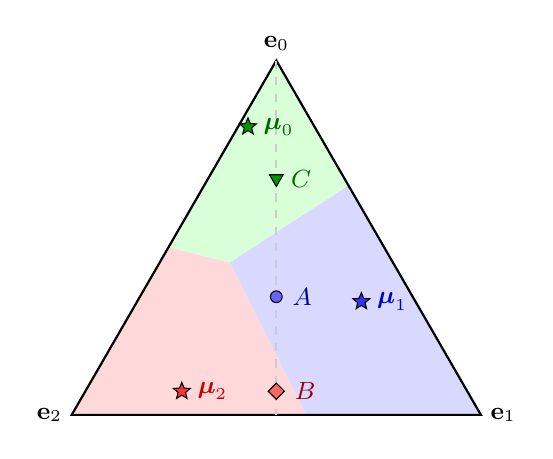
\begin{tikzpicture}[scale=0.6, font=\sffamily]

    % --- 1. Define Coordinates ---
    
    % The Triangle Vertices (Simplex)
    \coordinate (Top) at (0, 5);          
    \coordinate (Right) at (4.33, -2.5);  
    \coordinate (Left) at (-4.33, -2.5);  

    % The Prototypes (Stars)
    \coordinate (Mu0) at (-0.6, 3.6);    % Green (Top)
    \coordinate (Mu1) at (1.8, -0.1);    % Blue (Middle-Right)
    \coordinate (Mu2) at (-2.0, -2.0);   % Red (Bottom-Left)

    % The Data Points
    \coordinate (C) at (0, 2.5);   % Top Data
    \coordinate (A) at (0, 0);     % Middle Data
    \coordinate (B) at (0, -2.0);  % Bottom Data

    % --- 2. Background Regions (Voronoi Clipping) ---
    % Note: We draw these first so they are behind everything else
    
    % Region 0 (Green)
    \begin{scope}
        \clip (Top) -- (Right) -- (Left) -- cycle; 
        \path (Mu0) -- (Mu1) coordinate[midway] (M01);
        \clip ($(M01)!20cm!90:(Mu1)$) -- ($(M01)!20cm!-90:(Mu1)$) -- ($(M01)!20cm!180:(Mu1)$) -- cycle;
        \path (Mu0) -- (Mu2) coordinate[midway] (M02);
        \clip ($(M02)!20cm!90:(Mu2)$) -- ($(M02)!20cm!-90:(Mu2)$) -- ($(M02)!20cm!180:(Mu2)$) -- cycle;
        \fill[green!15] (-5,-5) rectangle (5,5);
    \end{scope}

    % Region 1 (Blue)
    \begin{scope}
        \clip (Top) -- (Right) -- (Left) -- cycle;
        \path (Mu1) -- (Mu0) coordinate[midway] (M10);
        \clip ($(M10)!20cm!90:(Mu0)$) -- ($(M10)!20cm!-90:(Mu0)$) -- ($(M10)!20cm!180:(Mu0)$) -- cycle;
        \path (Mu1) -- (Mu2) coordinate[midway] (M12);
        \clip ($(M12)!20cm!90:(Mu2)$) -- ($(M12)!20cm!-90:(Mu2)$) -- ($(M12)!20cm!180:(Mu2)$) -- cycle;
        \fill[blue!15] (-5,-5) rectangle (5,5);
    \end{scope}

    % Region 2 (Red)
    \begin{scope}
        \clip (Top) -- (Right) -- (Left) -- cycle;
        \path (Mu2) -- (Mu0) coordinate[midway] (M20);
        \clip ($(M20)!20cm!90:(Mu0)$) -- ($(M20)!20cm!-90:(Mu0)$) -- ($(M20)!20cm!180:(Mu0)$) -- cycle;
        \path (Mu2) -- (Mu1) coordinate[midway] (M21);
        \clip ($(M21)!20cm!90:(Mu1)$) -- ($(M21)!20cm!-90:(Mu1)$) -- ($(M21)!20cm!180:(Mu1)$) -- cycle;
        \fill[red!15] (-5,-5) rectangle (5,5);
    \end{scope}

    % --- 3. Draw Boundaries (Bisector Lines) ---
    % \begin{scope}
    %     \clip (Top) -- (Right) -- (Left) -- cycle;
    %     \draw[thick, green!50!black] ($(M01)!10cm!90:(Mu1)$) -- ($(M01)!10cm!-90:(Mu1)$);
    %     \draw[thick, blue!50!black] ($(M12)!10cm!90:(Mu2)$) -- ($(M12)!10cm!-90:(Mu2)$);
    %     \draw[thick, red!50!black] ($(M02)!10cm!90:(Mu2)$) -- ($(M02)!10cm!-90:(Mu2)$);
    % \end{scope}

    % --- 4. Main Triangle Frame & Blind Spot Line ---
    \draw[thick] (Top) -- (Right) -- (Left) -- cycle;
    \draw[dashed, gray!40, thick] (0, 5) -- (0, -2.5);

    % --- 5. Labels ---
    \node[above, font=\small] at (Top) {$\mathbf{e}_0$};
    \node[right, font=\small] at (Right) {$\mathbf{e}_1$};
    \node[left, font=\small] at (Left) {$\mathbf{e}_2$};

    % --- 6. Prototypes (Stars) ---
    \node[star, star points=5, star point ratio=2.25, fill=green!60!black, draw=black, inner sep=1pt] (Star0) at (Mu0) {};
    \node[right, green!40!black, font=\small\bfseries] at (Star0.east) {$\boldsymbol{\mu}_0$};
    
    \node[star, star points=5, star point ratio=2.25, fill=blue!80, draw=black, inner sep=1pt] (Star1) at (Mu1) {};
    \node[right, blue!80!black, font=\small\bfseries] at (Star1.east) {$\boldsymbol{\mu}_1$};
    
    \node[star, star points=5, star point ratio=2.25, fill=red!80, draw=black, inner sep=1pt] (Star2) at (Mu2) {};
    \node[right, red!80!black, font=\small\bfseries] at (Star2.east) {$\boldsymbol{\mu}_2$};

    % --- 7. Data Points ---
    % C (True: 0)
    \node[regular polygon, regular polygon sides=3, rotate=180, fill=green!60!black, draw=black, inner sep=1pt] (NodeC) at (C) {};
    \node[right, green!40!black, font=\small\bfseries] at (NodeC.west) {$C$};

    % A (True: 1)
    \node[circle, fill=blue!60, draw=black, inner sep=1.5pt] (NodeA) at (A) {};
    \node[right, blue!60!black, font=\small\bfseries] at (NodeA.east) {$A$};

    % B (True: 2)
    \node[diamond, fill=red!60, draw=black, inner sep=1.5pt] (NodeB) at (B) {};
    \node[right, red!60!black, font=\small\bfseries] at (NodeB.east) {$B$};

    % % --- 8. Legend ---
    % \matrix [draw, fill=white, fill opacity=0.9, anchor=south east, nodes={scale=0.8, anchor=west}] at (Right) {
    %     \node [regular polygon, regular polygon sides=3, rotate=180, fill=green!60!black, inner sep=1.5pt, label=right:Class 0] {}; \\
    %     \node [circle, fill=blue!60, inner sep=2pt, label=right:Class 1] {}; \\
    %     \node [diamond, fill=red!60, inner sep=2.5pt, label=right:Class 2] {}; \\
    %     \node [star, star points=5, fill=black, inner sep=2pt, label=right:Prototypes] {}; \\
    % };

\end{tikzpicture}
\end{document}
        \caption{Voronoi resolution of the vertical-stack configuration. Points $C, A, B$ lie along the altitude $p_1 = p_2$ that is invariant under the parallel-shift class-1-vs-2 score (Eq.~\ref{eq:vertical_stack_invariance}). Voronoi prototypes placed at distinct altitudes recover the correct partition into three horizontal strata.}\label{fig:voronoi_proof}
    \end{figure}

    Under $0/1$ loss, $\mathbf{c}_1 - \mathbf{c}_2 = (0, -1, 1)^\top$, so the difference between class-$1$ and class-$2$ parallel-shift scores is
    \begin{equation}\label{eq:vertical_stack_invariance}
        s_1(\mathbf{p}) - s_2(\mathbf{p}) = (\alpha_1 - \alpha_2) + (p_2 - p_1).
    \end{equation}
    Whenever $p_1 = p_2$ the cost terms of classes $1$ and $2$ coincide, so classifying $\mathbf{p}_A$ as $1$ forces $s_1(\mathbf{p}_A) \le s_2(\mathbf{p}_A)$, i.e.\ $\alpha_1 \le \alpha_2$, and classifying $\mathbf{p}_B$ as $2$ forces $\alpha_2 \le \alpha_1$. Both hold only if $\alpha_1 = \alpha_2$, whereupon $s_1 \equiv s_2$ on the altitude and $\mathbf{p}_A, \mathbf{p}_B$ receive the same label, so at least one of them is misclassified. Every parallel-shift rule therefore errs on at least one of the three points, giving $\inf_{\delta \in \mathcal{H}_{PS}} R(\delta) \ge 1/3 > 0$.

    Take $\boldsymbol{\mu}_0 = \mathbf{e}_0$, $\boldsymbol{\mu}_1 = (0.4, 0.5, 0.1)^\top$, $\boldsymbol{\mu}_2 = (0.1, 0.4, 0.5)^\top$. Direct computation shows~\eqref{eq:thm_vertex_consistency} holds for every $k$ (e.g., for $k = 1$, $\|\mathbf{e}_1 - \boldsymbol{\mu}_1\|_2^2 = 0.42 < 0.62 = \|\mathbf{e}_1 - \boldsymbol{\mu}_2\|_2^2 < 2 = \|\mathbf{e}_1 - \boldsymbol{\mu}_0\|_2^2$), so $\mathcal{M} \in \mathcal{H}_{Vor}^{\mathrm{DLC}}$. The squared distances at the two ambiguous points are
    \[
        d^2(\mathbf{p}_A, \boldsymbol{\mu}_1) = 0.08 < 0.14 = d^2(\mathbf{p}_A, \boldsymbol{\mu}_2), \qquad
        d^2(\mathbf{p}_B, \boldsymbol{\mu}_2) = 0.02 < 0.32 = d^2(\mathbf{p}_B, \boldsymbol{\mu}_1),
    \]
    so $\mathbf{p}_A \in \mathcal{P}_1^{\mathcal{M}}$ and $\mathbf{p}_B \in \mathcal{P}_2^{\mathcal{M}}$. At the third point $d^2(\mathbf{p}_C, \boldsymbol{\mu}_0) = 0.06 < 0.32 = d^2(\mathbf{p}_C, \boldsymbol{\mu}_1)$ and $< 0.74 = d^2(\mathbf{p}_C, \boldsymbol{\mu}_2)$, so $\mathbf{p}_C \in \mathcal{P}_0^{\mathcal{M}}$. All three points are thus classified to their true labels, so $R = 0$; since $\inf_{\delta \in \mathcal{H}_{PS}} R(\delta) \ge 1/3$, the strict separation $\inf_{\delta \in \mathcal{H}_{Vor}^{\mathrm{DLC}}} R(\delta) < \inf_{\delta \in \mathcal{H}_{PS}} R(\delta)$ follows. The Voronoi rule achieves this by placing prototypes at distinct altitudes, exploiting the $p_0$ direction that the parallel-shift score~\eqref{eq:vertical_stack_invariance} cannot see.
\end{proof}
